\usetikzlibrary{positioning,calc,fit}

\definecolor{black_red}{RGB}{179,0,0}
\definecolor{black}{RGB}{0,0,0}
\definecolor{blue}{RGB}{0,51,153}
\definecolor{orange}{RGB}{255,128,0}


\pgfdeclarelayer{core}
\pgfdeclarelayer{runtime}
\pgfsetlayers{core,main}

\pgfkeys{
  /tikz/node distance/.append code={
    \pgfkeyssetvalue{/tikz/node distance value}{#1}
  }
}

\newlength\myframesep
\setlength\myframesep{0pt}

\newcommand\widernode[5][core_node]{
\node[
        #1,
        inner sep=0pt,
        shift=($(#2.south)-(#2.north)$),
        yshift=-\pgfkeysvalueof{/tikz/node distance value},
        fit={(#2) (#3)},
        label=center:{\color{white}#4}] (#5) {};
}
% fix widernodeabove function, right now will shift nodes on X axis
\newcommand\widernodeabove[5][core_node]{
\node[
        #1,
        inner sep=0pt,
        shift=($(#2.north)+(#2.north)$),
        yshift=+\pgfkeysvalueof{/tikz/node distance value},
        fit={(#2) (#3)},
        label=center:{\color{white}#4}] (#5) {};
}

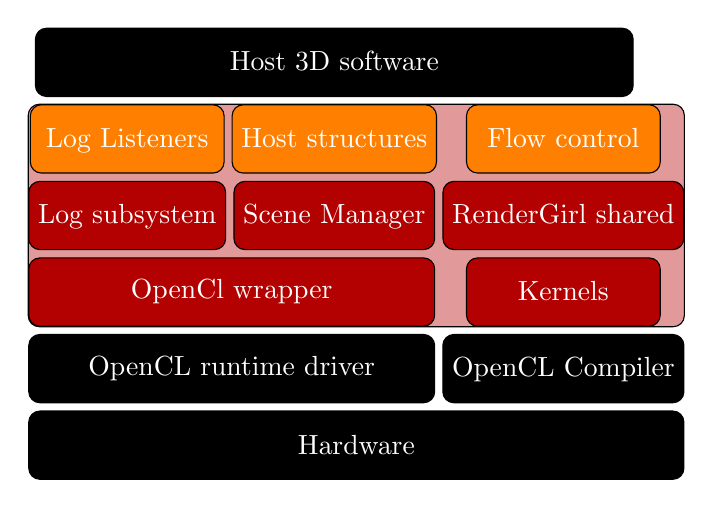
\begin{tikzpicture}[node distance=3pt,outer sep=0pt,
core_node/.style={
  draw=black,
  fill=black_red,
  rounded corners,
  font={\color{white}},
  align=center,
  minimum width = 70pt,
  text height=12pt,
  text depth=6pt},
other_node/.style={
  fill=black,
  draw=black,
  rounded corners,
  font={\color{white}},
  align=center,
  minimum width = 60pt,
  text height=12pt,
  text depth=6pt},
interface_node/.style={
  fill=orange,
  draw=black,
  rounded corners,
  font={\color{white}},
  align=center,
  minimum width = 70pt,
  text height=12pt,
  text depth=6pt},
host_node/.style={
  fill=black,
  draw=black,
  rounded corners,
  font={\color{white}},
  align=center,
  minimum width = 216pt,
  text height=12pt,
  text depth=6pt},
]

% core nodes

\node[core_node] (log) {Log subsystem};
\node[core_node, right=of log] (scene) {Scene Manager};
\node[core_node, right=of scene] (shared) {RenderGirl shared};
\widernode{log}{scene}{OpenCl wrapper}{wrapper};
\node[core_node, below=of shared] (kernels) {Kernels};

% interface

\node[interface_node, above=of scene](wrapper_host){Host structures};
\node[interface_node, above=of log](listeners){Log Listeners};
\node[interface_node, above=of shared](flow){Flow control};

\begin{pgfonlayer}{core}
\draw[core_node,draw=black,fill=black_red!40]
 ([xshift=-\myframesep,yshift=3\myframesep]current bounding box.north west)
    rectangle
  ([xshift=\myframesep,yshift=-\myframesep]current bounding box.south east);
\end{pgfonlayer}

% opencl runtime nodes

\widernode[other_node]{wrapper}{wrapper}{OpenCL runtime driver}{runtime}
\node[other_node, below=of kernels](compiler){OpenCL Compiler};

%  hardware

\widernode[other_node]{runtime}{compiler}{Hardware}{hardware}

% host 3d software

\node[host_node, above=of wrapper_host](host){Host 3D software};

\end{tikzpicture}